\documentclass[12pt]{article}
\usepackage[english,russian]{babel}
\usepackage{natbib}
\usepackage{vmargin}
\usepackage[utf8]{inputenc}
\usepackage{amsmath}
\usepackage{graphicx}
\graphicspath{{images/}}
\usepackage{parskip}
\usepackage{fancyhdr}
\setmarginsrb {3 cm} {2.5 cm} {3 cm} {2.5 cm} {1 cm} {1.5 cm} {1 cm} {1.5 cm}

\title{Проект базы данных для больницы}
\author{Мокеев Дмитрий}
\date{2020/2021}

\makeatletter
\let\thetitle\@title
\let\theauthor\@author
\let\thedate\@date
\makeatother

\pagestyle{fancy}
\fancyhf{}
\rhead{\theauthor}
\lhead{\thetitle}
\cfoot{\thepage}

\usepackage{natbib}
\usepackage{wasysym}
\usepackage{tikz}
\usetikzlibrary{arrows}
\usetikzlibrary{decorations.pathreplacing}
\usetikzlibrary{decorations.text}
\usepackage[T2A]{fontenc}
\usepackage{wrapfig}
\usepackage{mathrsfs}
\usepackage{color}
\usetikzlibrary{circuits}
\usetikzlibrary{circuits.ee}
\usetikzlibrary{circuits.ee.IEC}
\usetikzlibrary{circuits.logic.IEC}
\usepackage{rotating}
\usepackage{circuitikz} 
\usetikzlibrary{calc}
\usetikzlibrary{decorations}
\usetikzlibrary{decorations.pathmorphing}
\usetikzlibrary{positioning}
\usepackage{caption}
\captionsetup{labelsep=period}
\usepackage{pgfplots} 
\pgfplotsset{compat=1.7}
\graphicspath{{pic/}}

\begin{document}
	\begin{titlepage}
		\centering
		\vspace*{0.5 cm}
		
\includegraphics[width=5cm]{mipt_rus.png}\\[1.0 cm]	
		\textsc{\LARGE Московский физико-технический институт}\\[2.0 cm]	% University Name
		\textsc{\Large Базы Данных}\\[0.5 cm]				% Course Code
		\textsc{\large Курсовая работа}\\[0.5 cm]				% Course Name
		\rule{\linewidth}{0.2 mm} \\[0.4 cm]
		{ \huge \bfseries \thetitle}\\
		\rule{\linewidth}{0.2 mm} \\[1.5 cm]
		
		\begin{minipage}{0.4\textwidth}
			\begin{flushleft} \large
				\emph{Автор:}\\
				\theauthor
			\end{flushleft}
		\end{minipage}~
		\begin{minipage}{0.4\textwidth}
			\begin{flushright} \large
				\emph{Группа:} \\
				911									% Your Student Number
			\end{flushright}
		\end{minipage}\\[2 cm]
		
		{\large \thedate}\\[2 cm]
		
		\vfill
		
	\end{titlepage}

	\section{Проектирование}
	\subsection{Концептуальная модель}
	\begin{center}
		\begin{tikzpicture}
			\node[anchor=south west,inner sep=0] at (0,0) {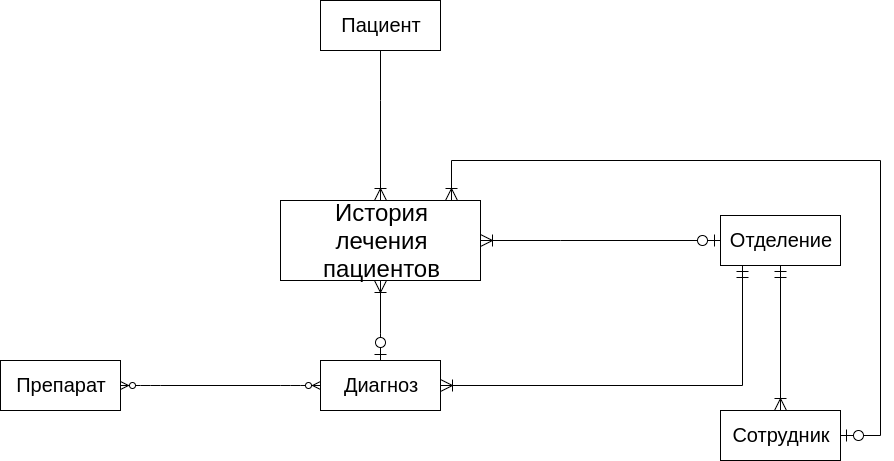
\includegraphics[width=15cm]{Концепт.png}};
		\end{tikzpicture}
	\end{center}
	В концептуальной модели базы данных основную роль выполняет история лечения пациентов, которая является сущностью, хранящую по сути попадания пациентов в больницу (приёмы и стационарное лечение).
	
	Отделение - это сущность-начальник для сотрудников, которые затем будут связаны с ним через вторичный ключ department id.
	
	В то же время отделение является родительской сущностью и для диагнозов. Эта связь сделана за желанием хранить в истории лечения идентификатор диагноза за редкостью обращения непосредственно к отделению (возможно, только в период составления отчётов по отделениям).
	
	Препараты являются небольшой вспомогательной сущностью для диагноза, связь многие ко многим. 
	
	Пациенты представляют собой людей, которые оказываются в этой базе данных, когда впервые попадают в больницу.
	
	Сотрудник --- это трудящийся в больнице, который может быть как врачом, так и нет, это сделано для упрощения модели базы данных.
	\subsection{Логическая модель}
	\begin{center}
		\begin{tikzpicture}
			\node[anchor=south west,inner sep=0] at (0,0) {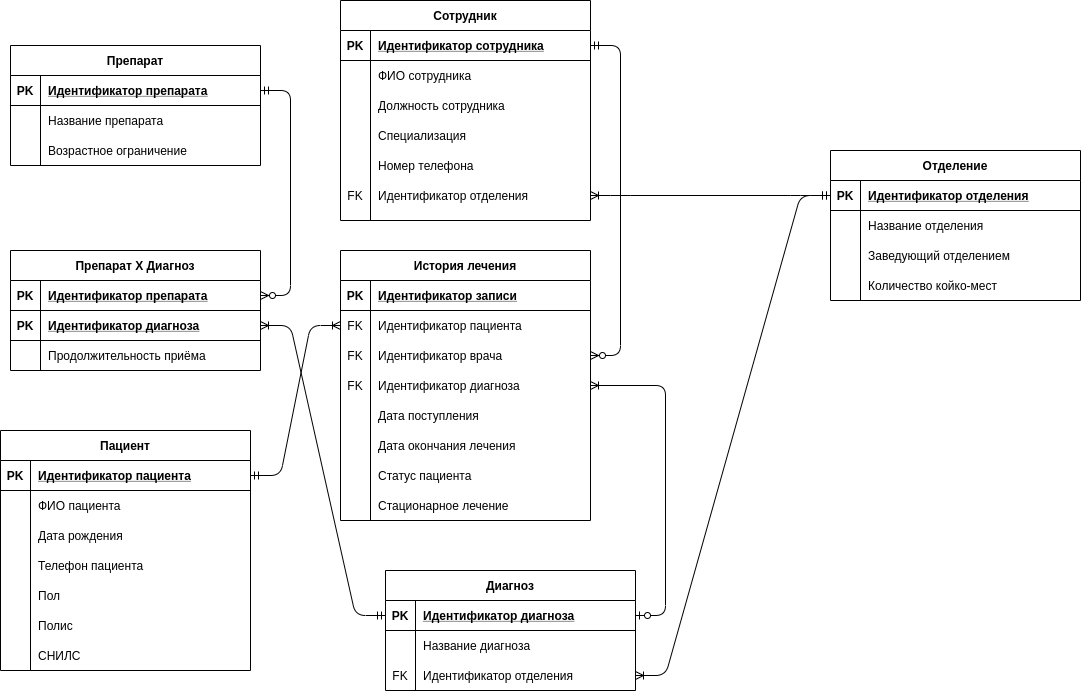
\includegraphics[width=15cm]{Логическая.png}};
		\end{tikzpicture}
	\end{center}
	В логической модели добавляется всего одна нужная таблица --- рвётся связь многие ко многим между препаратами и диагнозами. Почему так получилось? Потому что, к сожалению, объект истории лечения выполняется роль множественной связки и по сути это самая интересная таблица для какого-то анализа и запросов. В то же время она позволяется спастись от трёх отдельных и бессмысленных таблиц.
	
	Она в меру практична с человеческой точки зрения и её удобно заполнять врачам, что в принципе хорошо.
	При этом таблица находится в 2НФ, выбор обусловлен желанием данные вроде возрастного ограничения в одной таблице, не разрываясь из-за незначительных функциональных связей.
	\subsection{Физическая модель}
	\begin{center}
		\begin{tikzpicture}
			\node[anchor=south west,inner sep=0] at (0,0) {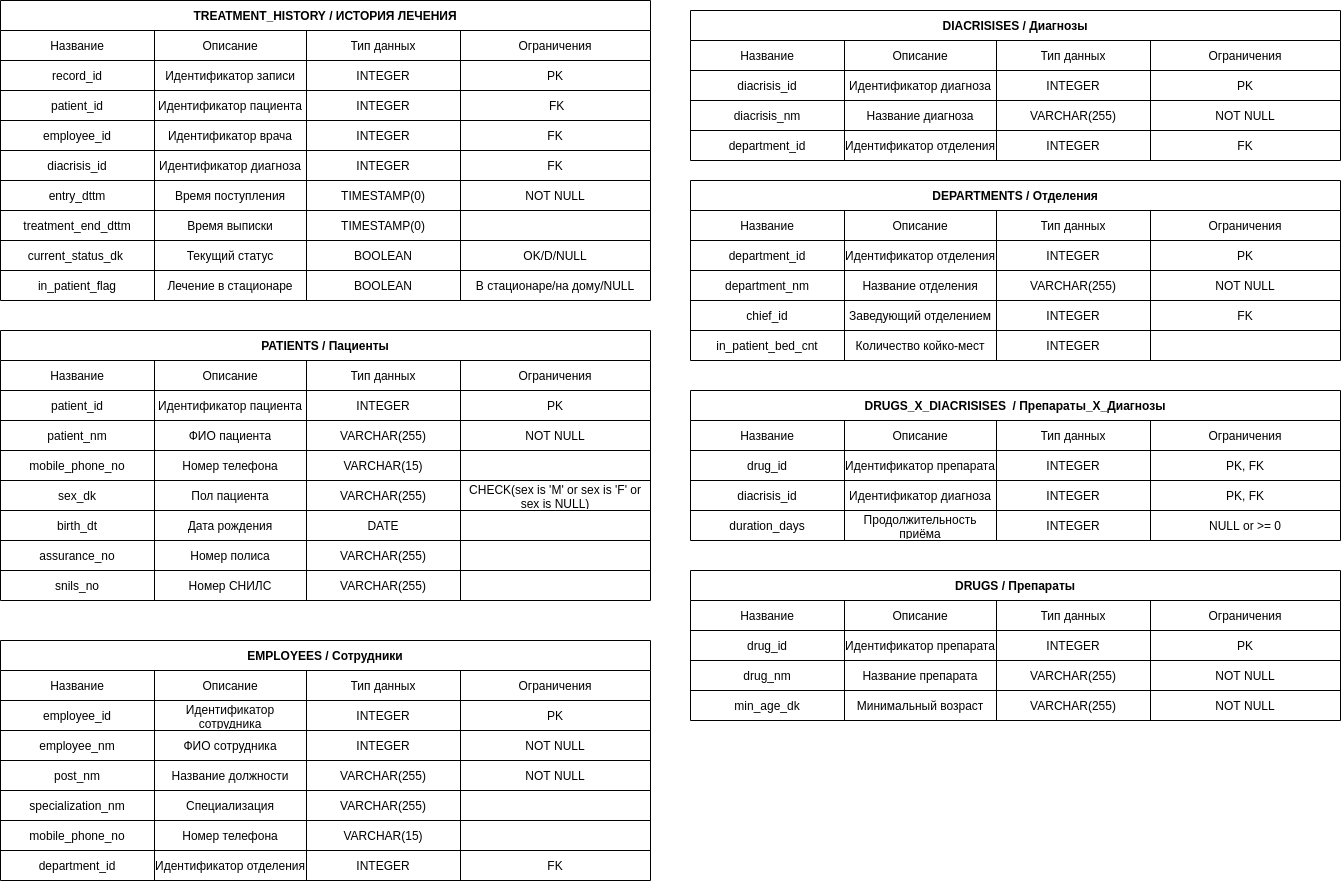
\includegraphics[width=15cm]{Физическая.png}};
		\end{tikzpicture}
	\end{center}
	Опишем непосредственно таблицы.
	
	\begin{enumerate}
		\item В таблице hospital.treatment\_history хранится информация о актах лечения в больнице.
		\item В таблице hospital.patients хранится информация о пациентах --- их идентификатор и личная информация. В этой таблице пациент оказывается прямо перед первой записью в историю лечения, что логично и соответствует реальности.
		\item В таблице hospital.\_employees хранятся данные о сотрудниках --- их рабочие и личные данные, а также номер отделения, выступающий в роли вторичного ключа для связи с отделениями.
		\item В таблице hospital.\_departments хранятся данные о отделениях, как о лечебных, так и не совсем --- например, о руководстве больницы. Заметим, что врач соответствует только одному отделению (в нашей модели). 
		\item В таблице hospital.\_drugs\_x\_diacrisises хранится связь между диагнозом и лекарством, а также время приёма лекарства для конкретного заболевания. Потенциально может быть добавлен ID для таблицы, в которой хранится некая вспомогательная информация.
		\item В таблице hospital.\_drugs хранится простейшая информация о лекарствах (можно добавить опцию количества имеющегося лекарства, но вообще база данных предназначена не для этого)
		\item В таблице hospital.\_diacrisises хранится информация о диагнозах --- по сути название и номер связанного с ним отделения.
	\end{enumerate}
	
	\section{Запросы}
	
	Опишем SELECT, следующие описывать не будем.
	\begin{enumerate}
		\item Определяет уровень смертности от COVID-19 в данной больнице за всё время ведения записи.
		\item Определяет, какие лекарства чаще всего используются при лечении пациентов в данной больнице и сколько раз они бывают нужны.
		\item Определяет случаи, когда в больницу попадает пациент, которого по бумагам нечем было лечить.
		\item Простой запрос: определяет всех пациентов фиксированного сотрудника и частоту их посещения.
		\item Определяет, сколько койко-мест занято в отделениях в фиксированное время.
	\end{enumerate}
	
\end{document}
